
\documentclass[11pt, letterpaper]{article}
%\usepackage{bookmark}
\usepackage[a4paper,margin=2cm]{geometry}
\usepackage[]{graphicx}
\usepackage{bm}
\usepackage[strings]{underscore}
\usepackage{apacite}
\setlength{\parindent}{0pt}
\graphicspath{ {./Images} }
\usepackage{wrapfig}
\usepackage[autostyle, english = american]{csquotes}
\usepackage[toc,page]{appendix}
\usepackage{amssymb}



\MakeOuterQuote{"}
\begin{document}
\begin{titlepage}
	\title{SOH-Coast-TOA: Modelling a roller coaster using trigonometric, cubic, and exponential functions}
	
	\author{Noah Alexiou}


	\date{March 2025}
	
	\maketitle
	\centering
	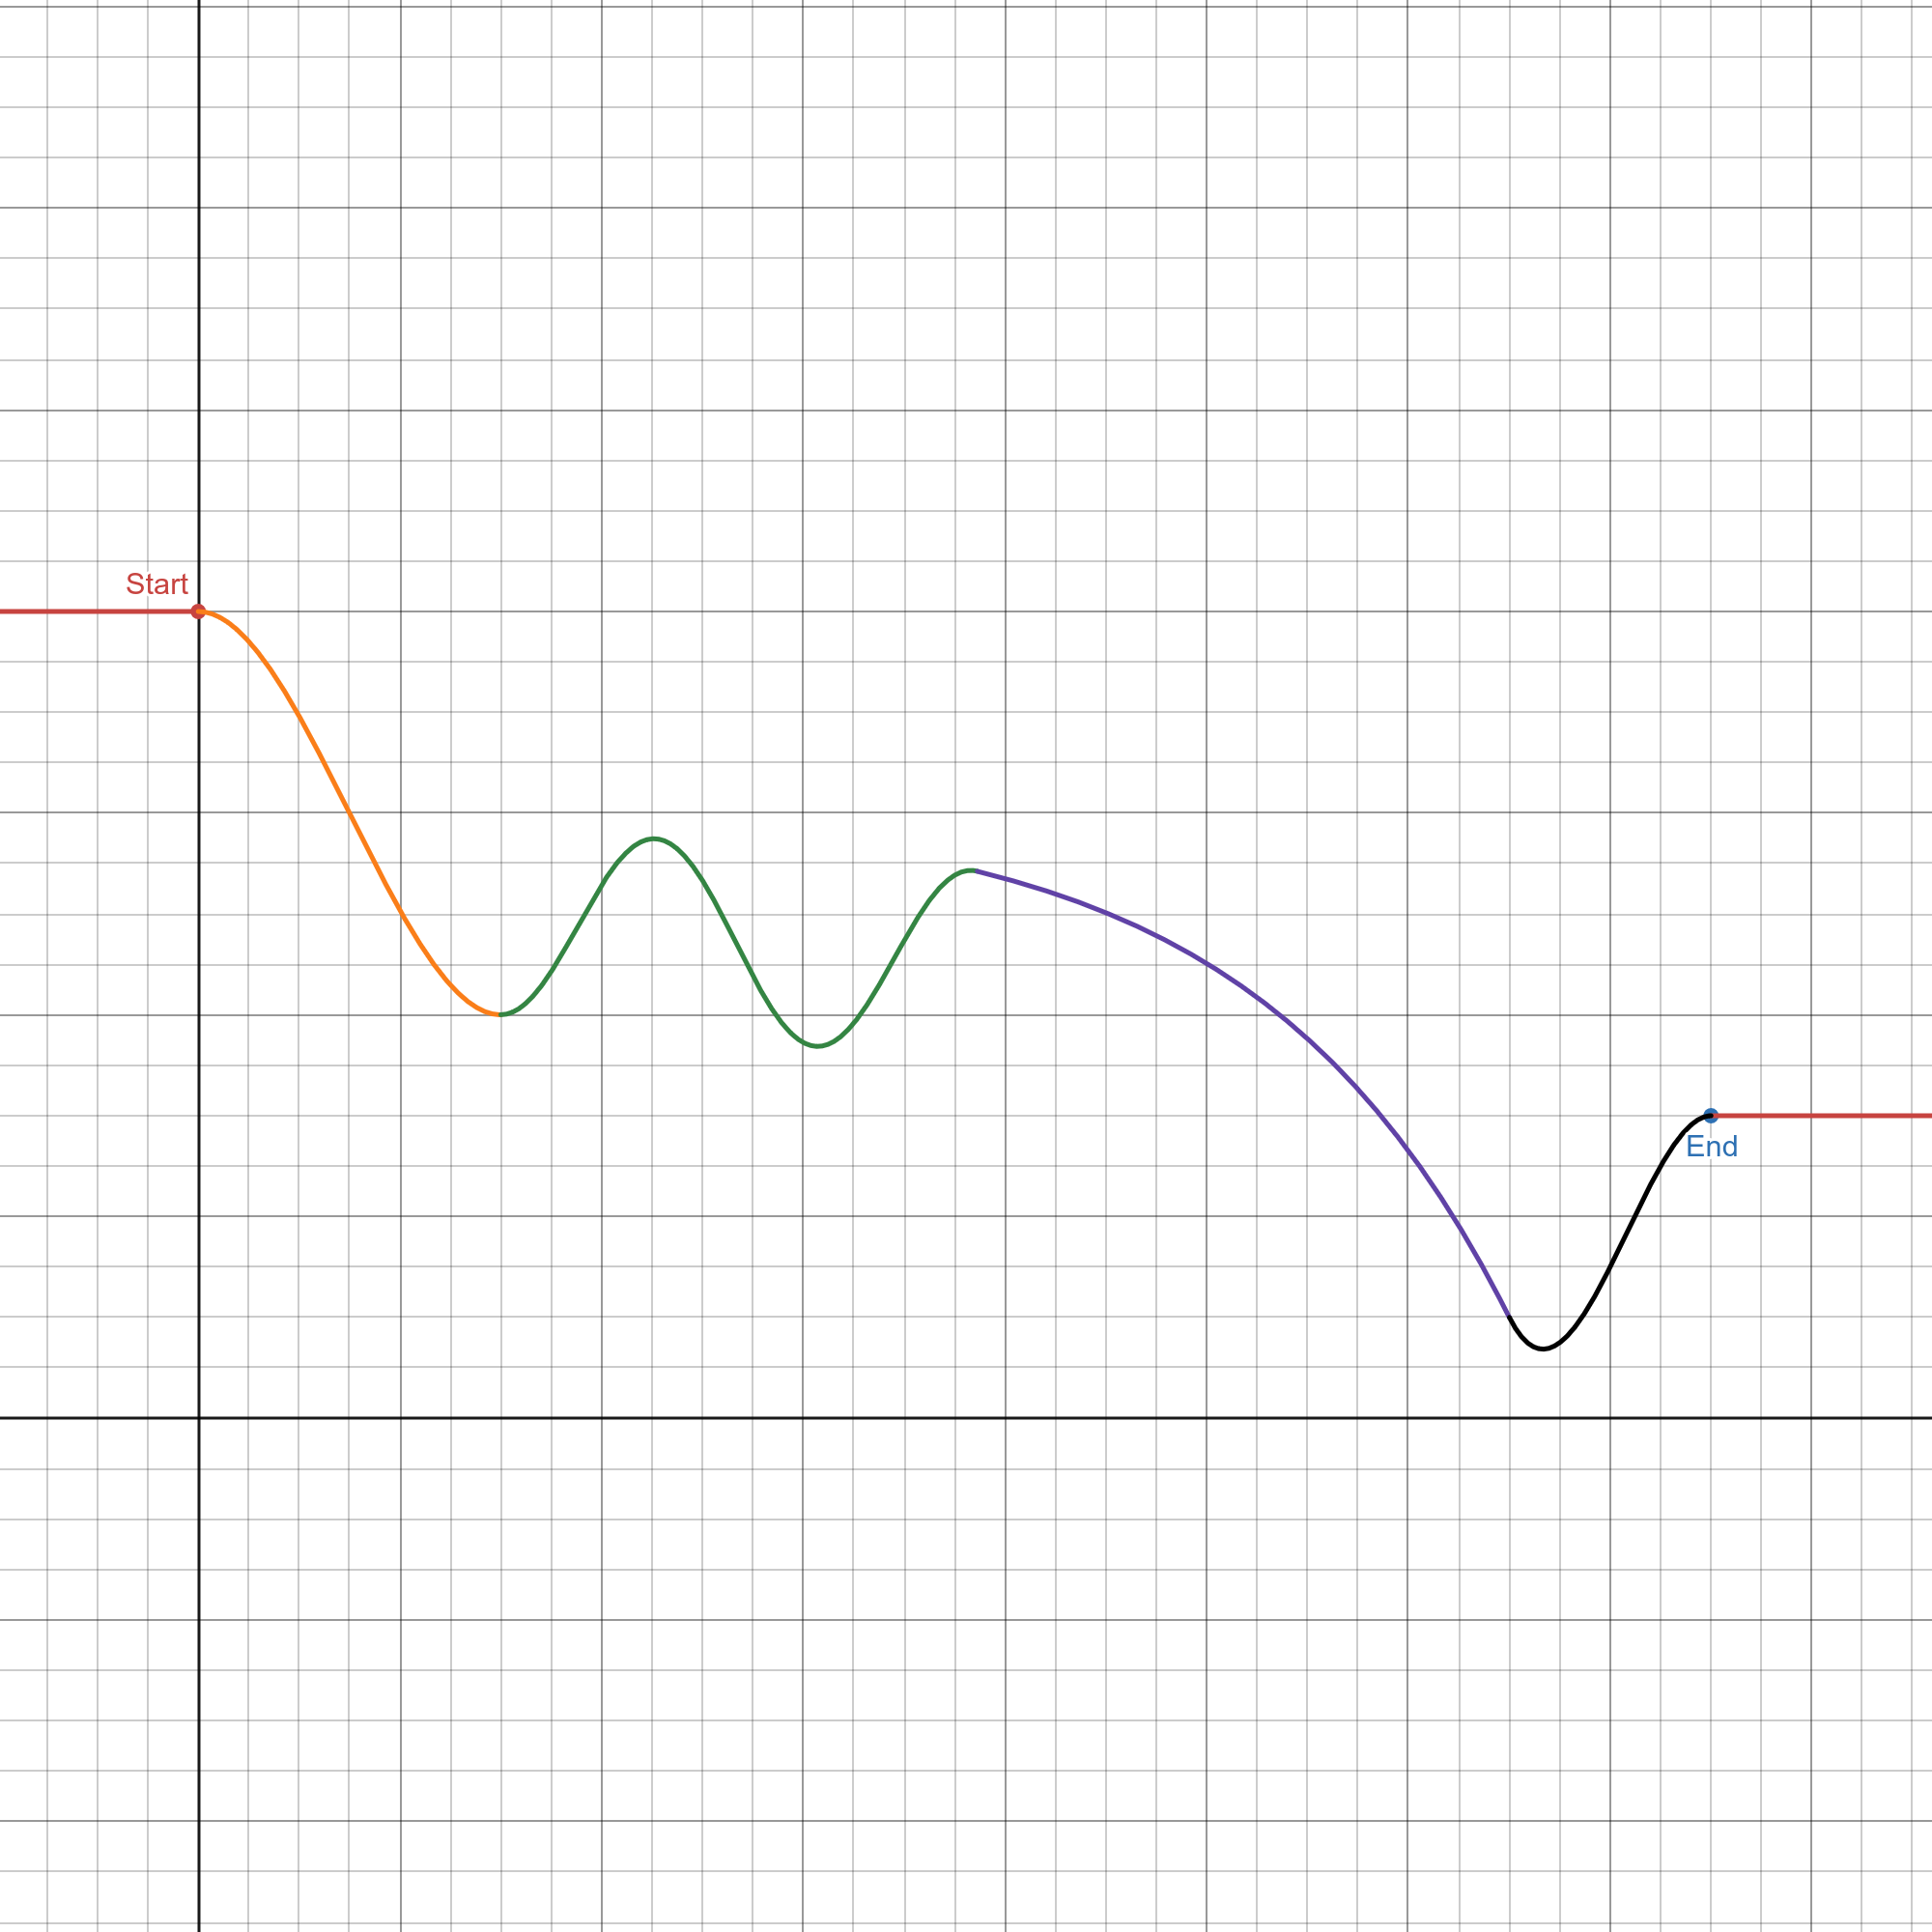
\includegraphics[width=1\linewidth]{finalgraph.png}
\begin{center}
	\large
	\vfill
	Maths Methods IA1
\end{center}
	
\end{titlepage}


\newpage
\tableofcontents


\newpage


\section{Formulation}
\subsection{Assumptions and Observations}


The terminology "smooth" was used to describe the required transition between pieces of track. It is assumed that this implied that at intersections, segments would be at same position, and have the same gradient.

The task sheet specified "The beginning and end sections... have been erected and are in a perfectly straight alignment". While this did clarify that the first, and end pieces of track were parallel, their slope was not specified, and therefore assumed to be 0.

For this task, the supporting structure under the track consists of equally spaced main columns priced at \$180/metre, and interconnecting bracing priced at \$20/metre$^2$. This lead to the assumption that placing support liberally to ensure sufficient integrity would be more cost effective than repairing catastrophic failure in the aftermath of improper placement.






		\begin{figure}[h]
	
	\begin{center}
		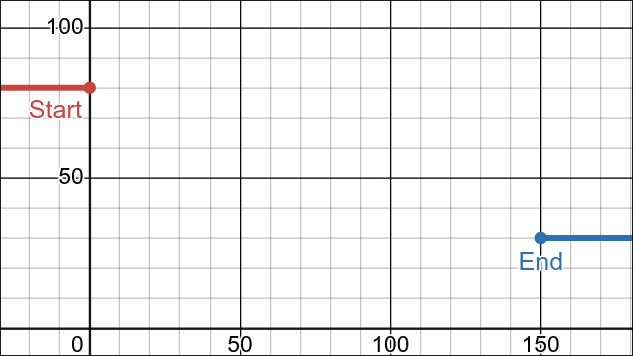
\includegraphics[width=15cm]{Start and End.png}
		
		\caption{The proposed start and end sections of the track}
	\end{center}
	
	
\end{figure}



The roller coaster was modelled in 2D to simplify calculations, and because graphing functions in 3D was out of the scope of the project. 


		
It was required that the track be constructed of at least 3 or more types of functions, including at least two types that are covered in Unit 3 Topic 2. The functions covered were exponential, logarithmic, and trigonometric functions.
	
Trigonometric functions were calculated in radians, rather than degrees, in order for them to naturally oscillate more with smaller change in $x$.

In order for the roller coaster to have sufficient speed to overcome any peaks or hills in the track, each successive peak should be at a lower height than any preceding it.

	




\subsection{Translation of aspects to Mathematical concepts and techniques}

Since the roller coaster had been assumed to be 2D, it's track was represented on the Cartesian plane. This allowed the use of desmos to graph its track and perform calculations by letting 1 unit be 1 meter. 

The derivative function of modelled sections of track could be used to determine the gradient at that specific points and therefore determine if the track exceeded the "maximum slope for safety" requirement provided by the task sheet. In this case, it was $-2$.

The task sheet defined the success criteria as maximising exhilaration, caused by "swift changes in direction, height and steepness". This could be could be translated to swift changes in the $y-$axis, and gradient.

In order to achieve as much of a thrill as possible, the maximum allowed slope should be reached whenever feasible while still incorporating change in gradient.
While the maximum slope is defined as $-2$, interpreting it directly as $-2\geq \textbf{slope}$ would result in a dangerously steep coaster that could only travel downwards. Henceforth any mention of a "maximum" or "highest possible" slope should be interpreted as the minimum slope so that $-2\leq \textbf{slope}$.




\section{Solve}
\subsection{Modelling in Desmos}
\subsubsection{The First Function}

Considering that the starting point of the first function was 80 meters in the air, there was already sufficient height for the maximum gradient to be reached for a reasonable duration.

Clearly the function will pass through point $(80, 0)$, therefore it is required that $f(0)=80$. So that there would be a smooth transition between track and function, it was required that for the cubic function, say $f(x)=ax^3 +bx^2 +cx +d$, $f'(0)=0$. Variables with $x$ coefficients become 0, Therefore $f'(0)=0\Rightarrow c=0$.

Since the derivative function was a quadratic, its lowest point could be considered the maximum slope reached by the original.

The $x$-coordinates of the turning point of a quadratic could found using the vertex formula, which stated that for turning point $(x, y),\; x=\frac{-b}{2a}$.

Considering the derivative function, $f'(x)=3ax^2+2bx$, it was found that the $x$-coordinates of the turning point were $\frac{-2b}{2\cdot3a}=\frac{-b}{3a}$.



\begin{figure}[h!]
	\centering
	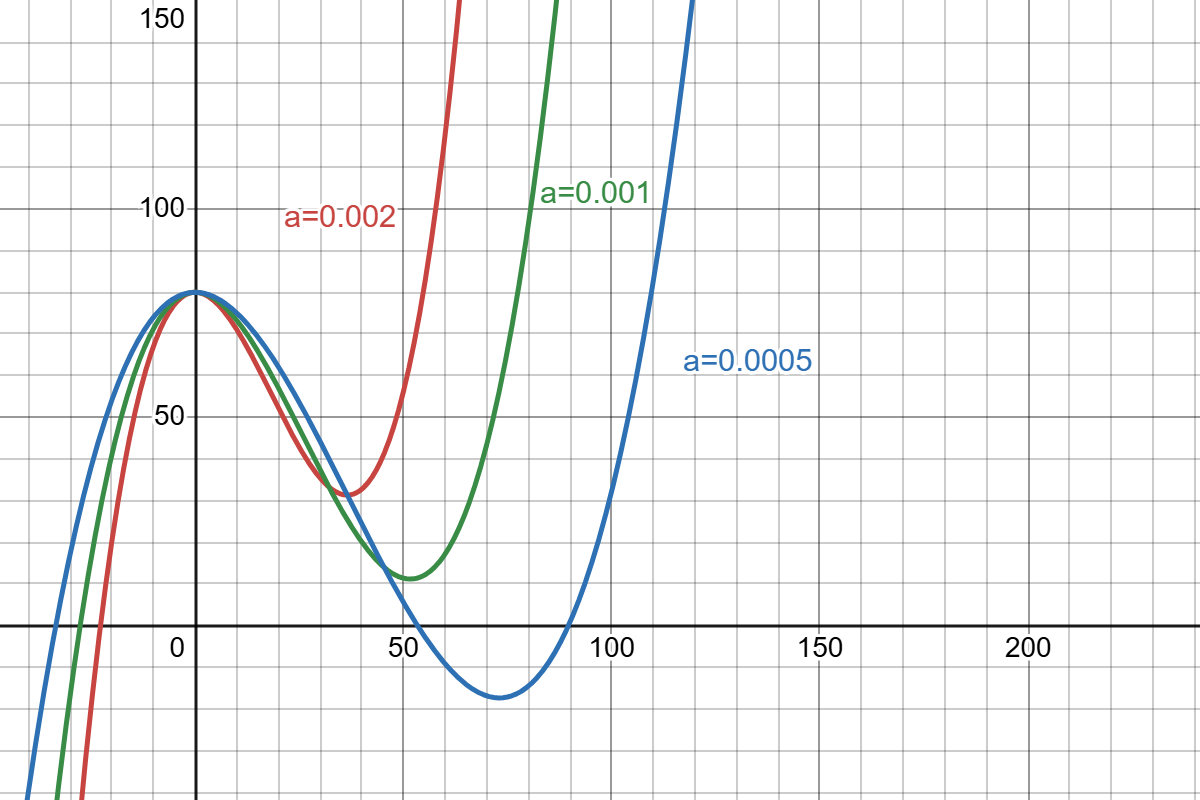
\includegraphics[width=15cm]{Eaxmple Cubic.png}
	\caption{Graphs of $f(x)=ax^{3}-\sqrt{6a}x^{2}+80$ with various $\mathbf{a}$ values}
\end{figure}


Therefore by finding $f'(\frac{-b}{3a})=-2$, a generic function could be found with minimum gradient -2, located at turning point. It was found that $f'(\frac{-b}{3a})=-2$ simplified to $b=\pm\sqrt{6a}$. Therefore the cubic $f(x)=ax^3\pm\sqrt{6a}x+d, a\geq0$ was found. 

$f(x)=ax^3-\sqrt{6a}x+80, a\geq0$ was inserted as it placed the "drop", and turning point on the right hand side of the start of the coaster, while smoothly connecting with the starting point. 


	


The end of the first function was chosen to be $f(30)$ to maintain sufficient altitude.

To make joining the next function easier, $f'(30)=0$ was considered. This indicated that:

$$a=\frac{2}{675}$$

$$\therefore f(x)=\frac{2}{675}x^{3}-\frac{2}{15}x^{2}+80$$


\subsubsection{The Second Function}
The sine function had potential for "swift changes in direction, height, and steepness". It was chosen to be the second function.

Consider $$s(x)=a\sin(b(x+c))+d \Rightarrow s'(x)=ab\cos(b(x+c))$$

Clearly the maximum downwards gradient was defined by $$ab\cdot-1,\;\;\;\;\; a,b \epsilon \mathbf{N}$$
and 
$$\cos(b(x+c))=-1$$

However the peak of the next oscillation would be the same height than the previous one. Therefore the function  had to be modified to ensure sufficient speed to overcome the next peak though the creation of a new function, $c(x)=a\sin(b(x+c))+d+gx$, so that $c'(x)=ab\cos(b(x+c))+g$. Clearly now when $g<0$, the function will slope downwards throughout its oscillation. 

	\begin{figure}[h!]
		\centering
		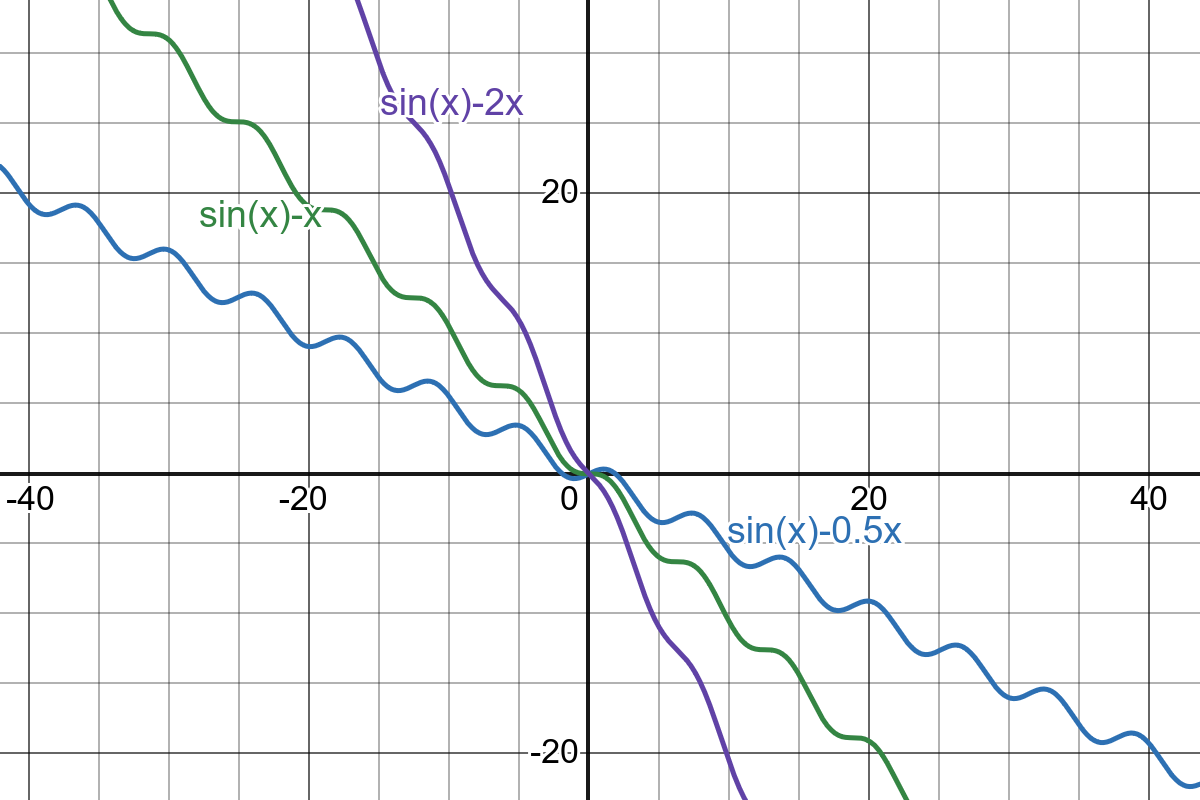
\includegraphics[width=15cm]{c(x).png}
		\caption{The function $y=sin(x)$ with various slopes applied}
	\end{figure}
	\pagebreak




Considering $g=-0.1$, clearly $ab\cdot -1-0.1=-2$ would result in a minimum gradient of $-2$. Through trial and error in Desmos it was found that for $c'(x)=-2$, $a=9.5$ and $b=0.2$ were appropriate. To align the functions, $f'(x)=c'(x)$ was considered. The function was shifted horizontally until the minimums were aligned, then shifted vertically using $d$ until the functions met.  

It was found  that $$9.5\cdot0.2\cos (0.2(30+c))-0.1=0 \Rightarrow c=-6.174775557$$

$$\therefore 9.5\sin(0.2(30-6.174775557))+d+3=40 \Rightarrow d=52.48683298$$

\subsubsection{The Third Function}
It was decided that the third function would be an exponential with decreasing gradient and height to utilize the remaining altitude and increase speed.

 Considering the general form of an exponential, $g(x)=ae^{b(x+c)}+d$, it was found that solving for variables $a, b, c$ and $d$ would require significant computation.

Therefore it was decided that by letting $c=0$, and $d=0$, only $a$ and $b$ would need to be solved for. 

Due to elimination of horizontal or vertical shifting, the point $(80, 0)$ was considered the origin for $g(x)$, so that  initial requirements such as $g(80)=c(80)$ became $g(0)=c(80)$. 

It was required that $$g'(0)=c'(80),g(0)=c(80), g'(50)=-2$$
Solving with simultaneous equations gave $$a=\frac{c'(80)}{be^{80b}}$$ 

$$\therefore g(80)=\frac{c'(80)}{be^{80b}}\cdot e^{80b}\Rightarrow b=\frac{c'(80)}{c(80)}\approx -0.023308398873$$

However this solution causes the exponential to intersect with the $x-\textrm{axis}$ prematurely. 
	\begin{figure}[h]
		\centering
		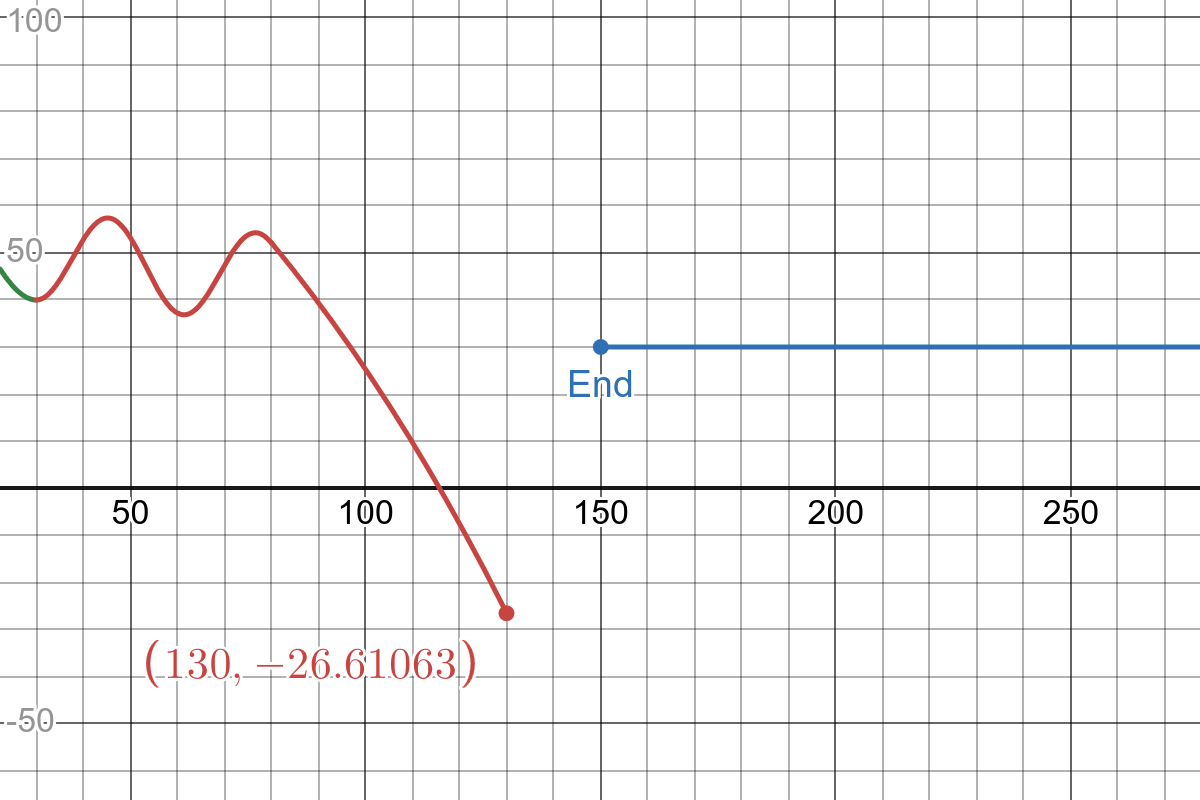
\includegraphics[width=15cm]{PrematureIntersecion.png}
		\caption{Graph of $g(x)$ prematurely intersecting with the $x-\textrm{axis}$}
	\end{figure}


	

By considering $s'(\lambda)=g'(0)$, a suitable $x$ value for the starting point of the function was defined, which did not cause contradictions when later conditions were established. 

This was rearranged to give $$a=\frac{s'(\lambda)}{b}$$

Substituting into $g'(\gamma)=-2$
 
 $$g'(\gamma)=-2=s'(\lambda)e^{\gamma b}\Rightarrow 
 b=\frac{1}{\gamma}\ln(\frac{-2}{s'(\lambda)})$$ Substituting into $g(x)=ae^{bx}$

 $$g(x)=\frac{s'(\lambda)}{\frac{1}{\gamma}\ln(\frac{-2}{s'(\lambda)})}\cdot e^{\frac{1}{\gamma}\cdot \ln (\frac{-2}{s'(\lambda)})\cdot x}$$ 
 
 where $\gamma$ is the distance that the function takes to reach $g'(x)=-2$, and $\lambda$ is the $x$ value that the joins with the previous function, $s(x)$.
		

$x$ was replaced with $(x-\lambda)$ horizontally shift, and $s(\lambda)-a$ was inserted at the end to vertically shift so that $g(\lambda)=s(\lambda)$.
		

After inserting the equation into desmos, suitable values for $\lambda$ and $\gamma$ were found. It was required that the equation terminate at $y=10$ so that there would be room for the final function to invert direction and climb. Therefore $g(\lambda + \gamma)=10$, where $\gamma=130-\lambda$, was considered, as this would ensure that $g'(\lambda-\lambda-130)=g'(130)=-2$, while still allowing for $\lambda$ to be altered until a suitable answer was found.
		

It was found that for $g'(130)=-2$ and $g(130)=10$, $\lambda=77.2487110854776$. Therefore $g(x)=\frac{s'(\lambda)}{\frac{1}{\gamma}\ln(\frac{-2}{s'(\lambda)})}\cdot e^{\frac{1}{\gamma}\cdot \ln (\frac{-2}{s'(\lambda)})\cdot (x-\lambda)}+s\left(\lambda\right)-\frac{s'(\lambda)}{\frac{1}{\gamma}}\ln\left(\frac{-2}{s'\left(\lambda\right)}\right)$ where $\lambda=77.2487110854776$, and $\gamma=130-\lambda$.





\subsubsection{The Fourth Function}

The final function was decided to be a cubic function, as multiple turning points were required, and the process for defining a cubic with constraints had already been established when creating the first function. 
	

It was required that for the cubic function, say $f_2(x)=a_2x^3+b_2x^2+c_2x+d_2$, $f_2'(130)=g'(130)$, $f_2(130)=g(130), f_2'(150)=0$, and $f_2(150)=30$. 
	
However to simplify calculations, it was considered that $f_2'(0)=g'(130)$, $f_2(0)=g(130), f_2'(20)=0$, and $f_2(20)=30$. Horizontal shift was later accounted for by substituting instances of $x$ with $(x-130)$
	

Solving simultaneously for these conditions gave values 
	
	$$a_{2}=\frac{g'\left(130\right)+40b_{2}}{-1200}$$
	
	$$b_{2}=\frac{3}{400}\cdot\left(30-\frac{g'\left(130\right)\cdot8000}{-1200}-\left(20\cdot g'\left(130\right)\right)-g\left(130\right)\right)$$
	
	$$c_{2}=g'\left(130\right)$$
	
	$$d_{2}=g\left(130\right)$$

For further working see appendix $\mathbf{A}$
	


\subsection{Final Functions and Domains}

$f_1$=


\subsection{Supporting Structures}
For this task, the supporting structure of roller coasters consists of equally spaced main columns priced at \$180/metre, and interconnecting bracing priced at \$20/metre$^2$.


\section{Evaluate and Verify}
\subsubsection{Reasonableness}



The assumption that the start and end pieces had a slope of 0 was found to be optimal for easily joining tracks to the  turning points of the inside functions. However, if it was instead assumed that the start and end pieces of track were slanted, with a gradient of, say $-2$, then the roller coaster would be more thrilling, as the passengers would be travelling faster and experience greater forces.


While simplification of the model to 2D did make the roller coaster less thrilling, as passengers would only experience thrilling movements in 2 dimensions, rather than 3, it greatly simplified calculations as intended


\subsubsection{Strengths}


The function $c(x)$ had the largest changes in gradient, which theoretically contributed the largest thrill to passengers. Additionally, it not only reached the maximum slope throughout its oscillation, but ensured that passengers maintained enough speed to overcome each one of its peaks through its integrated linear function.

While the cubic function was utilized heavily, the requirements for there to be at least two types of functions that were covered in Unit 3 Topic 2 included in the roller coaster and least 3 types of functions overall, were fulfilled.



\subsubsection{Limitations}


The organisation and labelling of functions and variables throughout the solution were inconsistent and confusing. A better naming scheme was adopted toward the end of the task, with the last function becoming $f_2(x)$, rather than an arbitrary letter. 

Many variables lacked exact solutions. This resulted in extremely long and complex functions which lacked readability and accuracy. While this was sub optimal, the rounding errors were found to be inconsequential considering the real world scale.

Cost of the attraction was considered when placing the supports after the design had been finalised, however cost was not considered during the design or refinement process. Lowering the coaster would result in lower support costs, but less of a thrill from the final drop down $g(x)$.

Being restricted to equally spaced main columns means that rather than placing fewer, but more intentionally placed, pillars, the amount of pillars had to be increased dramatically in order to support sections of the track that bear higher loads.
\section{Conclusion}
- briefly summarise some of the task and solution
- what we did
- how we did it
- total cost 

\begin{appendices}
	\section{The First Function}
	
	
	\section{The Fourth Function}
	$f_2(0)=g(130)\Rightarrow d=g(130)$
	
	$f_2'(0) = g'(130)\Rightarrow c=g'(130)$
	
	$f'(20)=0\Rightarrow a=1200a+40b+g'(130)$
	
	
\end{appendices}





\end{document}